\documentclass{beamer}

\usepackage[utf8]{inputenc}
\usepackage[english]{babel}
\usepackage{tikz}
\usepackage{mathtools}
\usepackage{multirow}
\usepackage{anyfontsize}
\graphicspath{{imgs/}}

\newcommand{\NN}{\ensuremath{\mathbb N}}
\newcommand{\ZZ}{\ensuremath{\mathbb Z}}
\newcommand{\QQ}{\ensuremath{\mathbb Q}}
\newcommand{\RR}{\ensuremath{\mathbb R}}
\newcommand{\CC}{\ensuremath{\mathbb C}}
\newcommand{\LL}{\ensuremath{\mathbb L}}
\newcommand{\PP}{\ensuremath{\mathbb P}}

\usetheme{Ilmenau}
\usecolortheme{beaver}

\setbeamerfont{itemize/enumerate subbody}{size=\scriptsize}

\newcommand{\unit}[1]{\ensuremath{\:\text{#1}}}
\newcommand{\pro}{\ensuremath{\unit{\%{}}}}

\expandafter\def\expandafter\insertshorttitle\expandafter{%
  \insertshorttitle\hfill%
  \insertframenumber\,/\,\inserttotalframenumber}

\setbeamertemplate{itemize item}[square]
\setbeamertemplate{itemize subitem}[circle]
\setbeamertemplate{enumerate item}[square]

\title{20 Raspberry Pi's, One Model}

\subtitle{
    Federated Learning On Real Hardware
}
\author[Søren Holm, Asger Schultz, Gustav Moesmand]
{Søren Winkel Holm, Asger Laurits Schultz, Gustav Lang Moesmand}
\institute[DTU]{Technical University of Denmark}
\date{\today}

\begin{document}
\begin{frame}
    \titlepage
\end{frame}

\begin{frame}
    \frametitle{The Presentation}
    \footnotesize
    \tableofcontents
\end{frame}

\section{The Federated Learning Problem}
\begin{frame}
\end{frame}

\section{FedAvg on Real Hardware}
\begin{frame}
    \frametitle{FedAvg: The Simple Algorithm}
    \begin{enumerate}
        \item Initialize global model, $\mathcal M_G$
        \item Distribute to $S<C$ clients
        \item On each client $s$, train local model $\mathcal M_s$ for $E$ epochs
        \item Aggregate models
    \begin{equation*}
        \mathcal M_G \gets \frac{1}{S} \sum_{s=1}^{S} \mathcal M_s
    \end{equation*}
        \item Repeat from step 2 for $L$ communication rounds
    \end{enumerate}
\end{frame}
\frame {
    \frametitle{A Real-Life Setup}
    \noindent
    \parbox[t]{6cm}{
        \begin{itemize}
            \item Most experiments focus only on performance under different hyperparameters
            \item Fail to capture tradeoffs in practical applications
            \item E.g. if few local epochs is better for convergence, is that worth additional overhead?
        \end{itemize}    
    }
    \hfill
    \raisebox{\dimexpr-\height+\baselineskip}{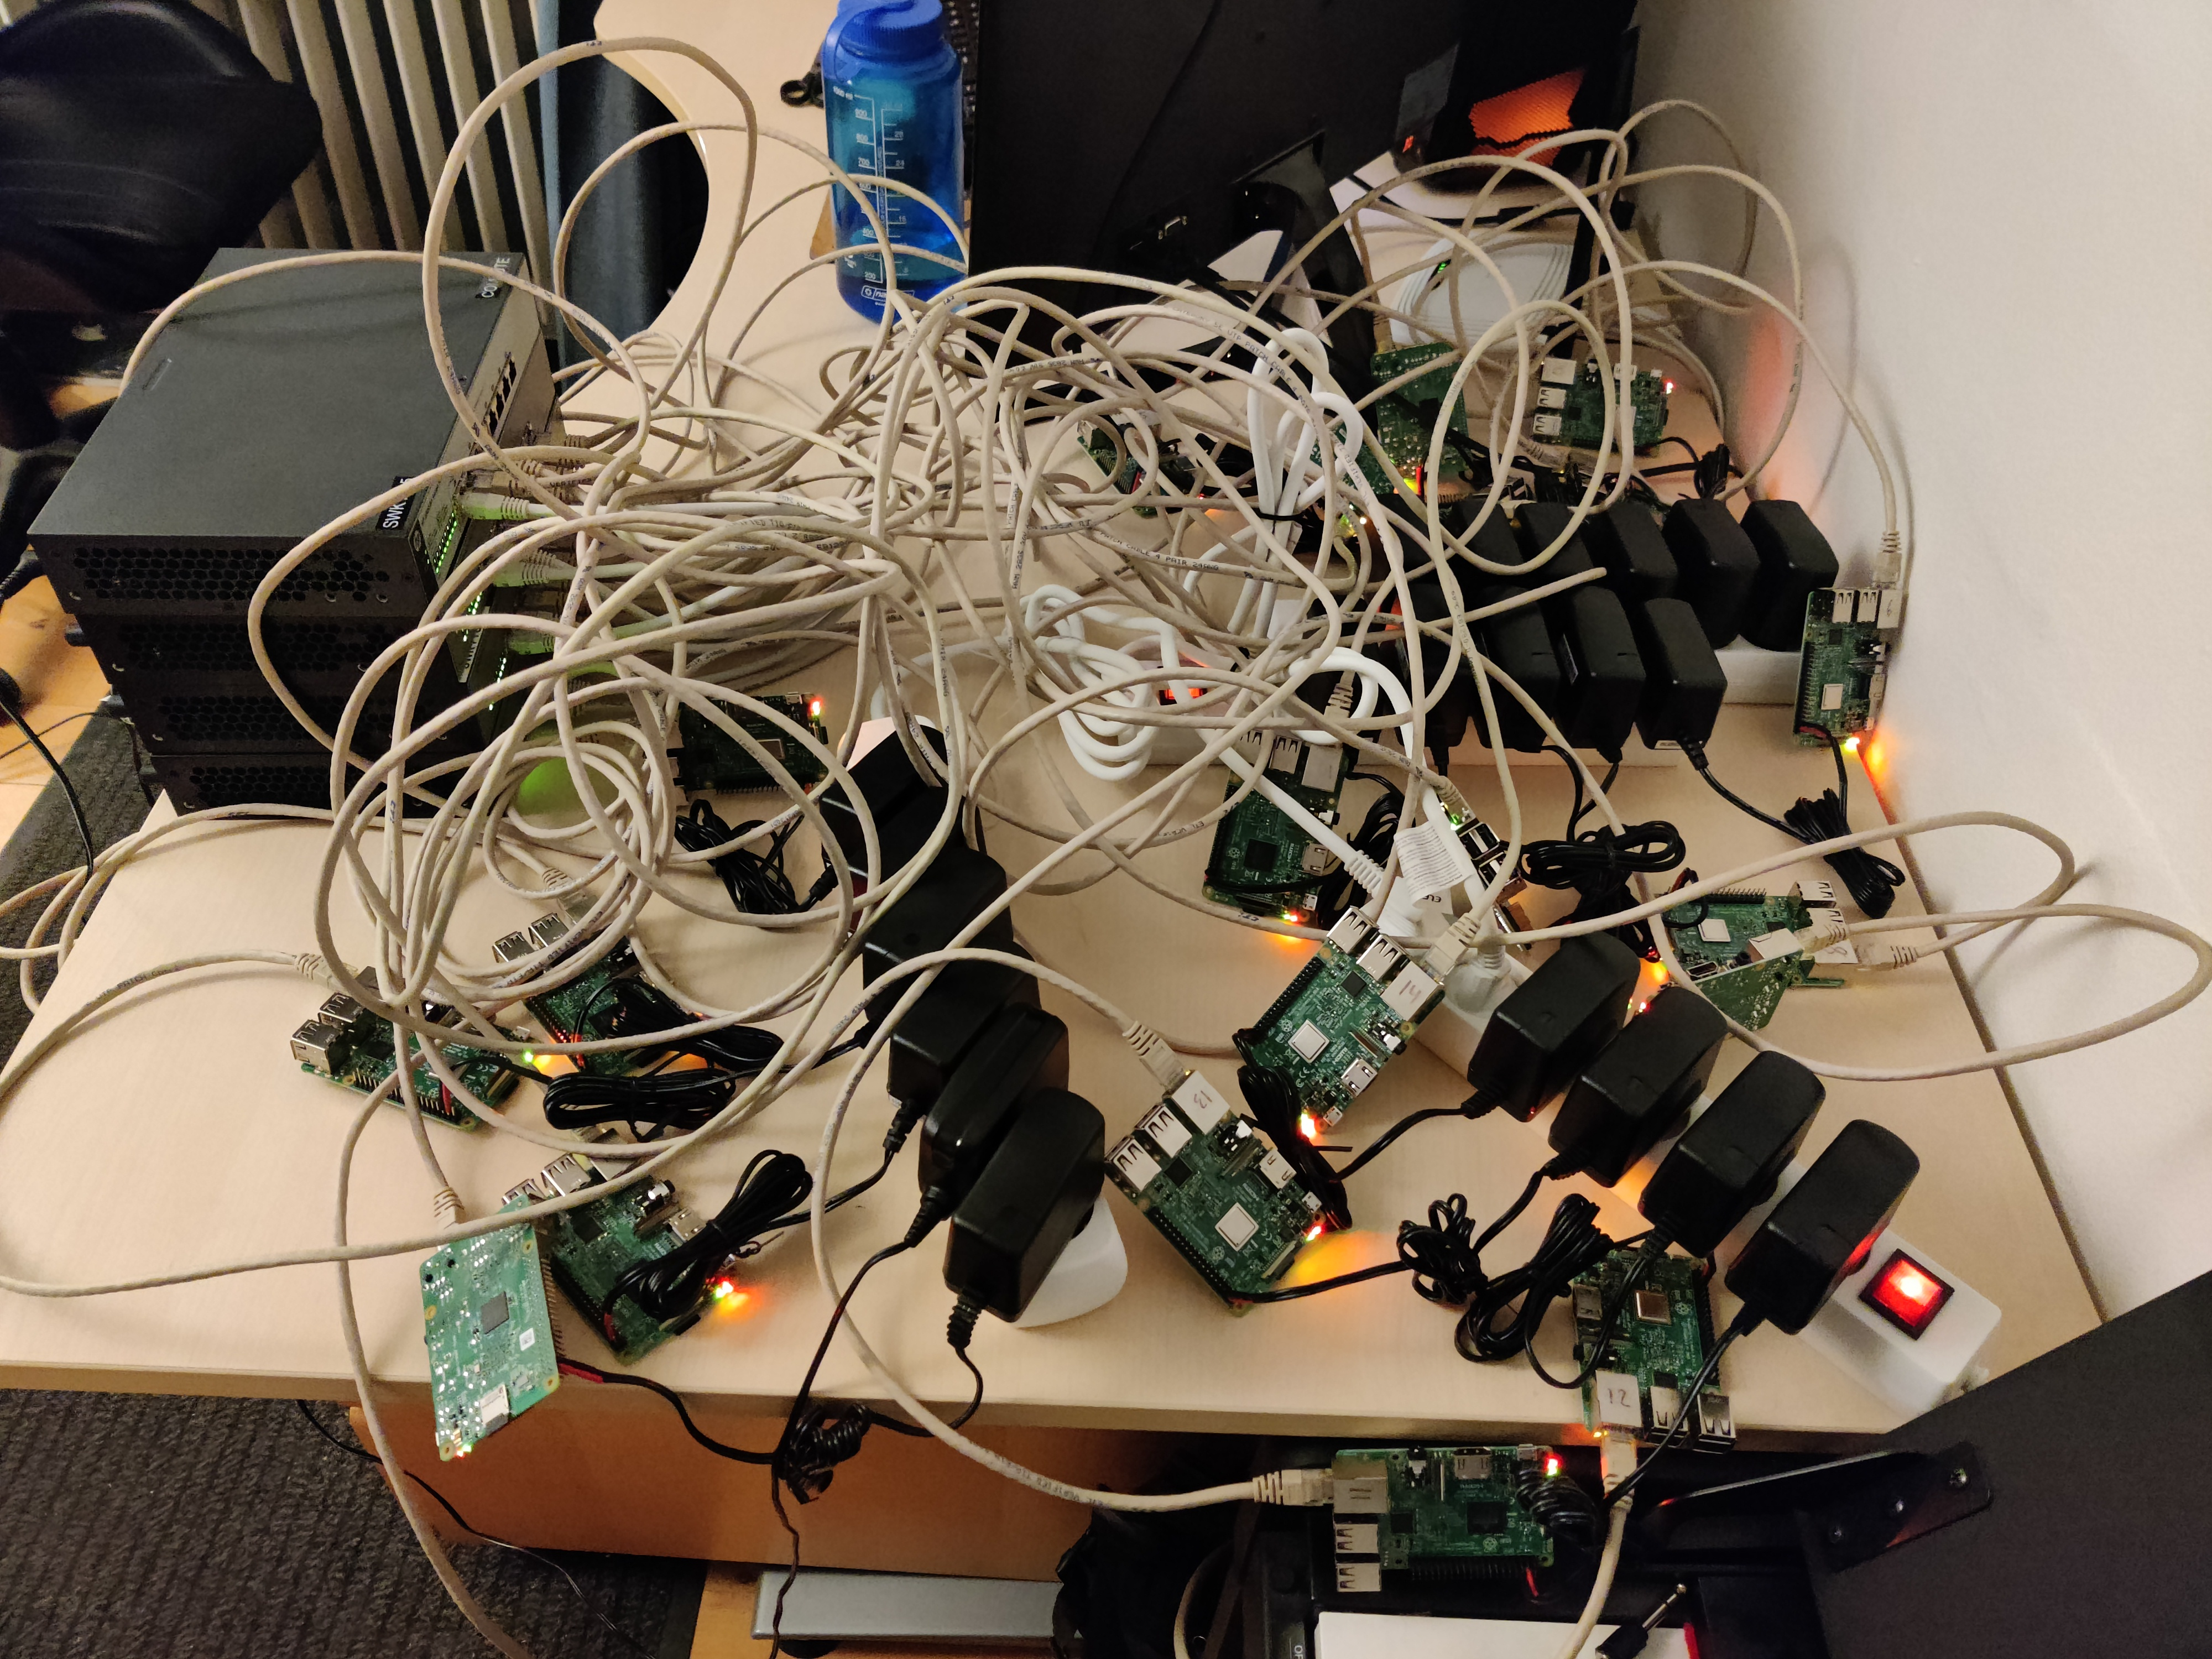
\includegraphics[width=.4\textwidth]{imgs/IMG_20220322_214443}}
}

\section{Robust Aggregation Using FedDF}
\begin{frame}
    \frametitle{Federated Robustness}
\end{frame}

\begin{frame}
    \frametitle{The FedDF Algorithm}
\end{frame}

\end{document}
